\section{Bất phương trình bậc nhất hai ẩn}

\subsection{Đề 1}
 \Opensolutionfile{ans}[ans/ans-0-C2-B1.D1-LC]
 \caulc
  \begin{ex}%[0D2H1-1]
 	Bất phương trình nào sau đây là bất phương trình bậc nhất hai ẩn?
 	\choice
 	{$\dfrac{-1}{7}x-\dfrac{y^2}{3} \le 8$ }
 	{$\sqrt{2} x^2-5 \sqrt{y} \ge 8$}
 	{$2 \cdot \dfrac{1}{x}-5\cdot \dfrac{1}{y}>8$}
 	{\True $-\dfrac{2}{5} x-5^2 y \leq-\sqrt{15}$}
 	\loigiai{
 		Bất phương trình bậc nhất hai ẩn là  $-\dfrac{2}{5} x-5^2 y \leq-\sqrt{15}$.
 	}
 \end{ex}
 
 \begin{ex}%[0D2H1-2]
 	Cho bất phương trình bậc nhất hai ẩn $2 x-5 y \leq 8$. Khẳng định nào dưới đây là khẳng định \textbf{sai}?.
 	\choice
 	{$(3 ;-4)$ là một nghiệm của bất phương trình}
 	{\True $(-2 ; 2)$ không là một nghiệm của bất phương trình}
 	{ $(-3 ;-1)$ là một nghiệm của bất phương trình}
 	{ $(5 ; 0)$ không là một nghiệm của bất phương trình}
 	\loigiai{
 		Thay $(-2 ; 2)$ vào bất phương trình $2 x-5 y \leq 8$ ta được $2 \cdot (-2)-5\cdot 2 \leq 8 \Leftrightarrow-14 \leq 8$
 		(đúng), nên $(-2 ; 2)$ là một nghiệm của bất phương trình $2 x-5 y \leq 8$.
 	}
 \end{ex}
 
 \begin{ex}%[0D2H1-2]
 	Cho bất phương trình $-2 x+3 y>3$. Khẳng định nào dưới đây \textbf{sai}?
 	\choice 
 	{$(0 ; 0)$ không là nghiệm bất phương trình}
 	{\True $(-1 ; 1)$ không là nghiệm bất phương trình}
 	{$(0 ; 1)$ không là nghiệm bất phương trình}
 	{ $(1 ; 3)$ là nghiệm bất phương trình}
 	\loigiai{
 		Thay $x=-1$, $y=1$ vào bất phương trình $2+3>3$ (đúng).\\
 		Vì vậy $(-1 ; 1)$ là nghiệm bất phương trình.
 	}
 \end{ex}
 
 \begin{ex}%[0D2H1-2]
 	Điểm $O(0 ; 0)$ thuộc miền nghiệm của bất phương trình nào dưới đây?
 	\choice
 	{$x+3 y+2 \le 0$}
 	{$x+y+2 \le 0$}
 	{\True $2 x+5 y-2<0$}
 	{$2 x+y<0$}
 	\loigiai{
 		Thay $x=y=0$, ta được $-2<0$ (đúng).\\
 		Vì vậy $O(0 ; 0)$ thuộc miền nghiệm.
 	}
 \end{ex}
 
 \begin{ex}%[0D2H1-2]
 	Khẳng định nào dưới đây là khẳng định \textbf{đúng}?
 	\choice 
 	{Cho bất phương trình $3-2 y>0$ có miền nghiệm là nửa mặt phẳng bờ $3-2 y=0$ chứa $O$ (kể cả bờ)}
 	{Cho bất phương trình $2 x+y>1$ có miền nghiệm là nửa mặt phẳng bờ $-2 x+y+1=0$ chứa $O$ (bỏ bờ)}
 	{Cho bất phương trình $-2 x+y+1 \le 0$ có miền nghiệm là nửa mặt phẳng bờ $-2 x+y+1=0$ chứa $O$}
 	{\True  Cho bất phương trình $2 x-3 y+5 \ge 0$ có miền nghiệm là nửa mặt phẳng bờ $2 x-3 y+5=0$ chứa $O$ (kể cả bờ)}
 	\loigiai{
 		Thay điểm $O(0;0)$ vào bất phương trình $2 x-3 y+5 \ge 0$, ta  được : $2\cdot 0-3\cdot 0 +5=5 \ge 0$ (đúng).
 	}
 \end{ex}
 
 \begin{ex}%[0D2H1-2]
 	Cho bất phương trình bậc nhất hai ẩn $x-2 y+2 \le 0$. Chọn khẳng định \textbf{sai }trong các khẳng định dưới đây?
 	\choice 
 	{Miền nghiệm của bất phương trình $x-2 y+2 \leq 0$ là nửa mặt phẳng không chứa bờ $d\colon x-2 y+2=0$, không chứa gốc tọa độ $O$}
 	{\True $(1;4)$ không là nghiệm của bất phương trình $x-2 y+2 \leq 0$}
 	{$(0 ; 3)$ không là nghiệm của bất phương trình $x-2 y+2 \leq 0$}
 	{ $(2 ; 2)$ không là nghiệm cùa bất phương trình $x-2 y+2 \leq 0$}
 	\loigiai{
 		
 		Thay điểm $(1;4)$ vào bất phương trình, ta được: $1\cdot 1-2\cdot 4+2=-5<0$ (đúng).\\
 		Vậy $(1;4)$ là nghiệm của bất phương trình $x-2 y+2 \le 0$.
 	}
 \end{ex}
 
 \begin{ex}%[0D2H1-2]
 	Cho bất phương trình $4 x-3 y \le 5\quad(\ast)$. Khẳng định nào dưới đây \textbf{đúng}?
 	\choice
 	{ $(1;-1)$ là nghiệm của bất phương trình $(\ast)$}
 	{$(0 ; 0)$ không là nghiệm của bất phương trình $(\ast)$}
 	{\True $(2 ; 1)$ là nghiệm của bất phương trình $(\ast)$}
 	{$(3 ;-1)$ là nghiệm của bất phương trình $(\ast)$}
 	\loigiai{
 		Thay $(2;1)$ vào bất phương trình ta được: $4\cdot 2-3\cdot 1=5\le 5$ (đúng) nên $(2 ; 1)$ là nghiệm của $4 x-3 y \leq 5$.
 	}
 \end{ex}
 
 \begin{ex}%[0D2N1-2]
 	Miền nghiệm của bất phương trình $3(x-1)+4(y-2)<5x-3$ là nửa mặt phẳng chứa điểm:
 	\choice
 	{$Q(-5;3)$}
 	{\True $O(0;0)$}
 	{$N(-4;2)$}
 	{$P(-2;2)$}
 	\loigiai{
 		Ta có : $3(x-1)+4(y-2)<5x-3\Leftrightarrow -x+2y-4<0\quad(\ast)$\\
 		Thay $O(0;0)$ vào $(\ast)$ ta được: $-0+1\cdot -4=-4<0$\\
 		Do đó: $O(0;0)$ thuộc miền nghiệm của bất phương trình.
 	}
 \end{ex}
 
 
 
 \begin{ex}%[0D2H1-2]
 	Đường thẳng $d\colon 2x-y=2$  chia mặt phẳng tọa độ thành hai miền I, II có bờ là đường thẳng $d$. Xác định miền nghiệm của bất phương trình $2x-y\ge 2$.
 	\begin{center}
 		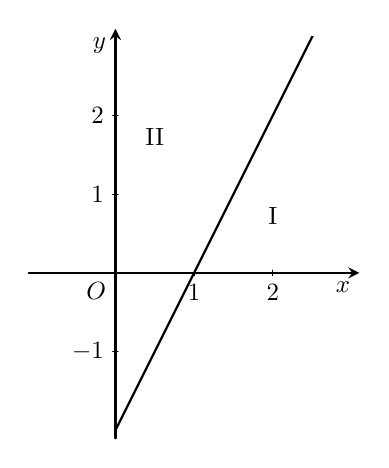
\begin{tikzpicture}[line join=round, line cap=round,>=stealth,thick]
 			\tikzset{every node/.style={scale=0.9}}
 			\draw[->] (-1.1,0)--(3.1,0) node[below left] {$x$};
 			\draw[->] (0,-2.1)--(0,3.1) node[below left] {$y$};
 			\draw (0,0) node [below left] {$O$};
 			\foreach \x/\nx in {1/1,2/2}
 			\draw[thin] (\x,1pt)--(\x,-1pt) node [below] {$\nx$};
 			\foreach \y/\ny in {-1/-1,1/1,2/2}
 			\draw[thin] (1pt,\y)--(-1pt,\y) node [left] {$\ny$};
 			\begin{scope}
 				\clip (-1,-2) rectangle (3,3);
 				\draw[samples=200,domain=-1:3,smooth,variable=\x] plot (\x,{2*(\x)+-2});
 			\end{scope}
 			\path (0.5,1.5)node [above]{II};
 			\path (2,0.5)node [above]{I};
 		\end{tikzpicture}
 	\end{center}
 	\choice
 	{Nửa mặt phẳng I bỏ đi đường thẳng $d$}
 	{\True Nửa mặt phẳng I kể cả bờ $d$}
 	{Nửa mặt phẳng II kể cả bờ $d$}
 	{Nửa mặt phẳng II bỏ đi đường thẳng $d$}
 	\loigiai{
 		Thay tọa độ điểm $O(0;0)$ vào bất phương trình đã cho, ta có $2\cdot -0\ge 2$ là mệnh đề sai. Do vậy miền nghiệm của bất phương trình đã cho là miền I không chứa điểm $O$, kể cả bờ $d$.
 	}
 \end{ex}
 
 
 \begin{ex}%[0D2H1-2]
 	Miền nghiệm được cho bởi hình bên là miềm nghiệm của bất phương trình nào dưới đây?
 	\begin{center}
 		\begin{tikzpicture}[line join=round, line cap=round,>=stealth,thick]
 			\tikzset{every node/.style={scale=0.9}}
 			\begin{scope}
 				\clip (-2,-1) rectangle (5,7);
 				\fill[pattern=north east lines] (-3,12)--(6,12)--(6,-6)--cycle;
 				\draw (-0.5,7)--(3.5,-1) node [pos=0.45, above, sloped] {$2x+y-6=0$};
 			\end{scope}
 			\draw[->] (-2,0)--(5,0) node[below]{$x$};
 			\draw[->] (0,-1)--(0,7) node[left]{$y$};
 			\draw (0,0) node[below left]{$O$};
 			\foreach \x in {3}
 			\draw[thin] (\x,1pt)--(\x,-1pt) node [below] {$\x$};
 			\foreach \y in {6}
 			\draw[thin] (1pt,\y)--(-1pt,\y) node [left] {$\y$};
 		\end{tikzpicture}
 	\end{center}
 	\choice
 	{$2x+y-6>0$}
 	{\True $2x+y-6<0$}
 	{$x+2y-6<0$}
 	{$x+2y-6>0$}
 	\loigiai{
 		Gọi đường thẳng $d\colon y=ax+b$\\
 		Thay hai điểm $(3;0)$ và $(0;6)$ vào $d$ ta được: $\heva{&3a+b=0\\&b=6}\Rightarrow\heva{&a=-2\\&b=6}$\\
 		Vậy $d\colon 2x+y-6=0$\\
 		Ta thấy $O(0;0)$ thuộc miềm nghiệm nên $2x+y-6<0$.
 	}
 \end{ex}
 
 \begin{ex}%[0D2H1-2]
 	Hình vẽ nào sau đây biểu diễn miền nghiệm của bất phương trình $2x-3y-6\le 0$?
 	\choice
 	{
 		\begin{tikzpicture}[line join=round, line cap=round,>=stealth,thick]
 			\tikzset{every node/.style={scale=0.9}}
 			\begin{scope}
 				\clip (-2,-3) rectangle (4,1.5);
 				\fill[pattern=north east lines] (-3,-4)--(6,-4)--(6,2)--cycle;
 				\draw (5.25,1.5)--(-1.5,-3) ;
 			\end{scope}
 			\draw[->] (-2,0)--(4,0) node[below]{$x$};
 			\draw[->] (0,-3)--(0,1.5) node[left]{$y$};
 			\draw (0,0) node[below left]{$O$};
 			\foreach \x in {-1,1,2,3}
 			\draw[thin] (\x,1pt)--(\x,-1pt) node [below] {$\x$};
 			\foreach \y in {-2,-1,1}
 			\draw[thin] (1pt,\y)--(-1pt,\y) node [left] {$\y$};
 		\end{tikzpicture}
 	}
 	{
 		\begin{tikzpicture}[line join=round, line cap=round,>=stealth,thick]
 			\tikzset{every node/.style={scale=0.9}}
 			\begin{scope}
 				\clip (-2,-1.5) rectangle (4,3);
 				\fill[pattern=north east lines] (-3,4)--(6,4)--(6,-2)--cycle;
 				\draw (-1.5,3)--(5.25,-1.5);
 			\end{scope}
 			\draw[->] (-2,0)--(4,0) node[below]{$x$};
 			\draw[->] (0,-1.5)--(0,3) node[left]{$y$};
 			\draw (0,0) node[below left]{$O$};
 			\foreach \x in {-2,-1,1,2,3}
 			\draw[thin] (\x,1pt)--(\x,-1pt) node [below] {$\x$};
 			\foreach \y in {-1,1,2}
 			\draw[thin] (1pt,\y)--(-1pt,\y) node [left] {$\y$};
 		\end{tikzpicture}
 	}
 	{\True
 		\begin{tikzpicture}[line join=round, line cap=round,>=stealth,thick]
 			\tikzset{every node/.style={scale=0.9}}
 			\begin{scope}
 				\clip (-2,-3) rectangle (4,1.5);
 				\fill[pattern=north east lines] (-3,-4)--(-3,2)--(6,2)--cycle;
 				\draw (5.25,1.5)--(-1.5,-3);
 			\end{scope}
 			\draw[->] (-2,0)--(4,0) node[below]{$x$};
 			\draw[->] (0,-3)--(0,1.5) node[left]{$y$};
 			\draw (0,0) node[below left]{$O$};
 			\foreach \x in {-1,1,2,3}
 			\draw[thin] (\x,1pt)--(\x,-1pt) node [below] {$\x$};
 			\foreach \y in {-2,-1,1}
 			\draw[thin] (1pt,\y)--(-1pt,\y) node [left] {$\y$};
 		\end{tikzpicture}
 	}
 	{
 		\begin{tikzpicture}[line join=round, line cap=round,>=stealth,thick]
 			\tikzset{every node/.style={scale=0.9}}
 			\begin{scope}
 				\clip (-2,-1.5) rectangle (4,3);
 				\fill[pattern=north east lines] (-3,4)--(-3,-2)--(6,-2)--cycle;
 				\draw (-1.5,3)--(5.25,-1.5);
 			\end{scope}
 			\draw[->] (-2,0)--(4,0) node[below]{$x$};
 			\draw[->] (0,-1.5)--(0,3) node[left]{$y$};
 			\draw (0,0) node[below left]{$O$};
 			\foreach \x in {-1,1,2,3}
 			\draw[thin] (\x,1pt)--(\x,-1pt) node [below] {$\x$};
 			\foreach \y in {-1,1,2}
 			\draw[thin] (1pt,\y)--(-1pt,\y) node [left] {$\y$};
 		\end{tikzpicture}
 	}
 	\loigiai{
 		Đường thẳng $2x-3y-6=0$  đi qua hai điểm $(0;-2)$, $(3;0)$  nên loại đáp án $B$ và $D$.\\
 		Mặt khác $O(0;0)$ không thỏa mãn $2x-3y-6\le 0$  nên chọn đáp án $C$.
 	}
 \end{ex}
 
 \begin{ex}%[0D2V1-3]
 	Một công ty viễn thông tính phí $1$ nghìn đồng mỗi phút gọi nội mạng và $2$ nghìn đồng mỗi phút gọi ngoại mạng. Gọi $x$ và $y$ lần lượt là số phút gọi nội mạng, ngoại mạng của Bình trong một tháng và Bình muốn số tiền phải trả cho tổng đài luôn thấp hơn $100$ nghìn đồng. Chọn khẳng định \textbf{sai}?
 	\choice 
 	{ Số tiền phải trả cho cuộc gọi nội mạng mỗi tháng là $x$ (nghìn đồng), số tiền phải trả cho cuộc gọi ngoại mạng mỗi tháng là $2 y$ (nghìn đồng). Điều kiện $x \in \mathbb{N}$, $y \in \mathbb{N}$}
 	{ Bất phương trình bậc nhất gồm hai ẩn số $x$, $y$ đã cho là $x+2 y<100$}
 	{$x=50$, $y=20$ nghiệm của bất phương trình bậc nhất gồm hai ẩn số $x, y$ đã cho}
 	{\True Miền nghiệm của bất phương trình bậc nhất gồm hai ẩn số $x$, $y$ đã cho là một hình vuông}
 	\loigiai{
 		Bất phương trình biểu diễn số tiền Bình phải trả cho tổng đài là $x+2y<100$.\\
 		Biểu diễn miền nghiệm của $(\ast)$ trên hệ trục tọa độ. \\
 		Ta thấy điểm $O(0 ; 0)$ thuộc miền nghiệm của $(\ast)$ do thay tọa độ $O$ vào  $(\ast)$ ta được $0<100$ (đúng).\\
 		Vậy miền nghiệm của bất phương trình $(\ast)$  là nửa mặt phẳng (không kể $d$) có chứa điểm $O$ (phần không gạch chéo trên hình).
 		\begin{center}
 			\begin{tikzpicture}[line join=round, line cap=round,>=stealth,thick]
 				\tikzset{every node/.style={scale=0.9}}
 				\begin{scope}
 					\clip (-1,-1) rectangle (5,3);
 					\fill[pattern=north east lines] (-3,3.5)--(7,3.5)--(7,-1.5)--cycle;
 					\draw (-2,3)--(6,-1) ;
 				\end{scope}
 				\draw[->] (-1,0)--(5,0) node[below]{$x$};
 				\draw[->] (0,-1)--(0,3) node[left]{$y$};
 				\draw (0,0) node[below left]{$O$};
 				\foreach \x in {}
 				\draw[thin] (\x,1pt)--(\x,-1pt) node [below] {$\x$};
 				\foreach \y in {}
 				\draw[thin] (1pt,\y)--(-1pt,\y) node [left] {$\y$};
 				\draw (4,0) node [below] {$100$} node[above] {$B$} (0,2) node [right] {$50$}  node[left] {$A$};	
 			\end{tikzpicture}
 		\end{center}
 		Trong thực tế, vì $x \in \mathbb{N}$, $y \in \mathbb{N}$ nên ta chỉ xét miền nghiệm bất phương trình ứng với miền tam giác $O A B$.
 	}
 \end{ex}
\Closesolutionfile{ans}
\indapan{6}{ans/ans-0-C2-B1.D1-LC}
 \cauds
\Opensolutionfile{ans}[ans/ans-0-C2-B1.D1-DS]
 \begin{ex}%[0D2H1-2]
 	Cho điểm $(-1 ; 2)$ và các bất phương trình $3 x-5 y<-15$, $2 x+y \le 0$, $ 3 x-9 y>7$, $-4 x+3 y \ge 5$. Khi đó
 	\choiceTF
 	{\True $(-1 ; 2)$ không là một nghiệm của bất phương trình $3 x-5 y<-15$}
 	{\True $(-1 ; 2)$ là một nghiệm của bất phương trình $2 x+y \le 0$}
 	{$(-1 ; 2)$ là một nghiệm của bất phương trình $3 x-9 y>7$}
 	{\True $(-1 ; 2)$ là một nghiệm của bất phương trình $-4 x+3 y \ge 5$}
 	\loigiai{
 		\begin{itemchoice}
 			\itemch Đúng.\\
 			Thay $(-1 ; 2)$ vào bất phương trình $3 x-5 y<-15$ ta được \\
 			$3 \cdot ( -1)-5 \cdot 2<-15 \Leftrightarrow-13<-15$ (vô lí), nên $(-1 ; 2)$ không là một nghiệm của bất phương trình $3 x-5 y<-15$.
 			\itemch Đúng.\\
 			Thay $(-1 ; 2)$ vào bất phương trình $2 x+y \leq 0$ ta được $2 \cdot(-1)+2 \leq 0 \Leftrightarrow 0 \leq 0$
 			(đúng), nên $(-1 ; 2)$ là một nghiệm của bất phương trình $2 x+y \leq 0$.
 			\itemch Sai.\\
 			Thay $(-1 ; 2)$ vào bất phương trình $3 x-9 y>7$ ta được $3 \cdot (-1)-9 \cdot 2>7 \Leftrightarrow-21>7$
 			(vô lí), nên $(-1 ; 2)$ không là một nghiệm của bất phương trình $3 x-9 y>7$.
 			\itemch Đúng.\\
 			Thay $(-1 ; 2)$ vào bất phương trình $-4 x+3 y \geq 5$ ta được $-4 \cdot (-1)+3\cdot 2 \geq 5 \Leftrightarrow
 			10 \geq 5$ (đúng), nên $(-1 ; 2)$ là một nghiệm của bất phương trình $-4 x+3 y \geq 5$.
 	\end{itemchoice}}
 \end{ex}
 
 \begin{ex}%[0D2H1-1]
 	Xác định tính đúng, sai của các khẳng định sau.
 	\choiceTF 
 	{\True Miền nghiệm của các bất phương trình $6 x-y \leq 1$ chứa điểm $O$}
 	{Miền nghiệm của các bất phương trình $2 x+3 y>5$ chứa điểm $O$}
 	{\True Miền nghiệm của các bất phương trình $-3 x+y \geq 0$ chứa điểm $M(0 ; 1)$}
 	{\True Miền nghiệm của các bất phương trình $x-y<7$ chứa điểm $O$}
 	\loigiai{
 		\begin{itemchoice}
 			\itemch $6 x-y \leq 1$.\quad $(1)$\\
 			Vẽ đường thẳng $d\colon 6 x-y=1$ với các cặp giá trị là $x=0$, $y=-1$ và $x=\dfrac{1}{6}$, $y=0$.\\
 			Xét điểm $O(0 ; 0)$ thay $x=0$, $y=0$ vào $(1)$, ta được $0 \leq 1$ (đúng).\\
 			Do đó điểm $O$ thuộc miền nghiệm của $(1)$.\\
 			Vậy miển nghiệm của  $(1)$ là nửa mặt phắng (kế cả $d$)
 			chứa điểm $O$ (phần không gạch chéo trong hình).
 			\begin{center}
 				\begin{tikzpicture}[line join=round, line cap=round,>=stealth,thick]
 					\tikzset{every node/.style={scale=0.9}}
 					\begin{scope}
 						\clip (-3,-3) rectangle (3,3);
 						\fill[pattern=north east lines] (-4,-25)--(4,-25)--(4,23)--cycle;
 						\draw (0.67,3)--(-0.33,-3) ;
 					\end{scope}
 					\draw[->] (-3,0)--(3,0) node[below]{$x$};
 					\draw[->] (0,-3)--(0,3) node[left]{$y$};
 					\draw (0,0) node[below left]{$O$};
 					\foreach \y in {-1}
 					\draw[thin] (1pt,\y)--(-1pt,\y) node [left] {$\y$};
 				\end{tikzpicture}
 			\end{center}
 			\itemch  $2 x+3 y>5$.\quad $(2)$\\
 			Vẽ đường thẳng $d\colon 2 x+3 y=5$ với các cặp giá trị là $x=1$, $y=1$ và $x=\dfrac{5}{2}$, $y=0$.\\
 			Xét điểm $O(0 ; 0)$. Thay $x=0$, $y=0$ vào $(2)$, ta được $0>5$ (sai).\\
 			Do đó điểm $O$ không thuộc miền nghiệm của $(2)$.\\
 			Vậy miền nghiệm của $(2)$ là nửa mặt phẳng (không kể cả $ d$) không chứa điểm $O$ (phần không gạch chéo trong hình).
 			\begin{center}
 				\begin{tikzpicture}[line join=round, line cap=round,>=stealth,thick]
 					\tikzset{every node/.style={scale=0.9}}
 					\begin{scope}
 						\clip (-3,-3) rectangle (3,3);
 						\fill[pattern=north east lines] (-4,4.33)--(-4,-3.67)--(8,-3.67)--cycle;
 						\draw (-2,3)--(7,-3);
 					\end{scope}
 					\draw[->] (-3,0)--(3,0) node[below]{$x$};
 					\draw[->] (0,-3)--(0,3) node[left]{$y$};
 					\draw (0,0) node[below left]{$O$};
 				\end{tikzpicture}
 			\end{center}
 			\itemch $-3 x+y \geq 0$.\quad
 			$(3)$\\
 			Vẽ đường thẳng $d\colon -3 x+y=0$ với các cặp giá trị $x=0$, $y=0$ và $x=1$, $y=3$.\\
 			Xét điểm $M(0 ; 1)$; thay $x=0, y=1$ vào $(3)$ ta được $1 \geq 0$ (đúng), suy ra $M$ thuộc miền nghiệm của $(3)$.\\
 			Vậy miền nghiệm của $(3)$ là nửa mặt phẳng (kể cả $d$) chứa điểm $M$ (phần không gạch chéo trong hình).
 			\begin{center}
 				\begin{tikzpicture}[line join=round, line cap=round,>=stealth,thick]
 					\tikzset{every node/.style={scale=0.9}}
 					\begin{scope}
 						\clip (-2,-2) rectangle (2,2);
 						\fill[pattern=north east lines] (-3,-9)--(3,-9)--(3,9)--cycle;
 						\draw (0.67,2)--(-0.67,-2) ;
 					\end{scope}
 					\draw[->] (-2,0)--(2,0) node[below]{$x$};
 					\draw[->] (0,-2)--(0,2) node[left]{$y$};
 					\draw (0,0) node[below left]{$O$};
 				\end{tikzpicture}
 			\end{center}
 			\itemch $x-y<7$.\quad $(4)$\\
 			Vẽ đường thẳng $d\colon x-y=7$ với các cặp giá trị $x=7$, $y=0$ và $x=0$, $y=-7$.\\
 			Xét điểm $O(0 ; 0)$  thay $x=0$, $y=0$ vào $(4)$ ta được $0<7$ (đúng), suy ra $O$ thuộc miền nghiệm của $(4)$.\\
 			Vậy miền nghiệm của $(4)$ là nửa mặt phẳng (không kể $d$) chứa điểm $O$ (phần không gạch chéo trong hình).
 			\begin{center}
 				\begin{tikzpicture}[line join=round, line cap=round,>=stealth,thick]
 					\tikzset{every node/.style={scale=0.9}}
 					\begin{scope}
 						\clip (-1,-8) rectangle (8,1);
 						\fill[pattern=north east lines] (-2,-9)--(9,-9)--(9,2)--cycle;
 						\draw (8,1)--(-1,-8);
 					\end{scope}
 					\draw[->] (-1,0)--(8,0) node[below]{$x$};
 					\draw[->] (0,-8)--(0,1) node[left]{$y$};
 					\draw (0,0) node[below left]{$O$};
 					\foreach \x in {7}
 					\draw[thin] (\x,1pt)--(\x,-1pt) node [below] {$\x$};
 					\foreach \y in {-7}
 					\draw[thin] (1pt,\y)--(-1pt,\y) node [left] {$\y$};
 				\end{tikzpicture}
 			\end{center}
 		\end{itemchoice}
 	}
 \end{ex}
 
 
 \begin{ex}%[0D2H1-3]
 	An thích ăn hai loại trái cây là cam và xoài, mỗi tuần mẹ cho An $200\,000$ đồng để mua trái cây. Biết rằng giá cam là $15\,000$ đồng/kg, giá xoài là $30\,000$ đồng/kg. Gọi $x$, $y$ lần lượt là số kilôgam cam và xoài mà An có thể mua về sử dụng trong một tuần. Khi đó
 	\choiceTF 
 	{\True Trong tuần, số tiền An có thể mua cam là $15\,000x$, số tiền An có thể mua xoài là $30\,000 y$, ($x$, $y>0$)}
 	{Bất phương trình bậc nhất cho hai ẩn $x$, $y$ là $3 x+6 y \geq 40$}
 	{\True Cặp số $(5 ; 4)$ thỏa mãn bất phương trình bậc nhất cho hai ẩn $x$, $ y$}
 	{An có thể mua $4 $ kg cam, $5 $ kg xoài trong tuần}
 	\loigiai{
 		\begin{itemchoice}
 			\itemch Đúng. Trong tuần, số tiền An có thể mua cam là $15\,000 x$, số tiền An có thể mua xoài là $30\,000 y$ ($x$, $y>0$).
 			\itemch Sai. Ta có bất phương trình $15\,000 x+30\,000 y \leq 200\,000 \Leftrightarrow 3 x+6 y \leq 40$.\quad $(\ast)$
 			\itemch Đúng. Xét $x=5$, $y=4$, thay vào bất phương trình $3\cdot5+6\cdot 4 \leq 40$ (đúng) nên $(5 ; 4)$ là một nghiệm của $(\ast)$.
 			\itemch Sai. An có thể mua $5 $ kg cam, $4 $ kg xoài trong tuần.
 		\end{itemchoice}
 	}
 \end{ex}
 
 \begin{ex}%[0D2H1-3]
 	Một cửa hàng dành tối đa $10$ triệu để nhập $x$ tạ gạo và $y$ tạ mì. Biết mỗi tạ gạo mua hết $1{,}5$ triệu, mỗi tạ mì mua hết $1{,}2$ triệu. Khi đó
 	\choiceTF 
 	{\True Bất phương trình biểu thị mối liên hệ giữa $x$ và $y$ là $1{,}5 x+1{,}2 y \leq 10$}
 	{Bất phương trình biểu thị mối liên hệ giữa $x$ và $y$ là $1{,}5 x+1{,}2 y \geq 10$}
 	{\True Miền nghiệm của bất phương trình $1{,}5 x+1{,}2 y \leq 10$ là nửa mặt phẳng bờ là đường thẳng $(d)\colon 1{,}5 x+1{,}2 y=10$ chứa điểm $O(0 ; 0)$}
 	{Miền nghiệm của bất phương trình $1{,}5 x+1{,}2 y \leq 10$ là nửa mặt phẳng bờ là đường thẳng $(d)\colon 1{,}5 x+1{,}2 y=10$ không chứa điểm $O(0 ; 0)$}
 	\loigiai{
 		Bất phương trình biểu thị mối liên hệ giữa $x$ và $y$ là $1{,}5 x+1{,}2 y \leq 10$.\\
 		Miền nghiệm của bất phương trình $1{,}5 x+1{,}2 y \leq 10$ là nửa mặt phẳng bờ
 		là đường thẳng $(d)\colon 1{,}5 x+1{,}2  y=10$ chứa điểm $O(0 ; 0)$, được biểu diễn là miền không bị gạch chéo, tính cả bờ $(d)\colon 1{,}5 x+1{,}2 y=10$.
 		\begin{center}
 			\begin{tikzpicture}[line join=round, line cap=round,>=stealth,thick,scale=0.7]
 				\tikzset{every node/.style={scale=0.9}}
 				\begin{scope}
 					\clip (-2,-2) rectangle (10,10);
 					\fill[pattern=horizontal lines] (-3,12.08)--(11,12.08)--(11,-5.42)--cycle;
 					\draw (-1.33,10)--(8.27,-2) node [pos=0.45, below, sloped] {$1.5x+1.2y-10=0$};
 				\end{scope}
 				\draw[->] (-2,0)--(10,0) node[below]{$x$};
 				\draw[->] (0,-2)--(0,10) node[left]{$y$};
 				\draw (0,0) node[below left]{$O$};
 				\foreach \x in {7}
 				\draw[thin] (\x,1pt)--(\x,-1pt) node [below] {$\x$};
 				\foreach \y in {9}
 				\draw[thin] (1pt,\y)--(-1pt,\y) node [left] {$\y$};
 			\end{tikzpicture}
 		\end{center}
 	}
 \end{ex}
 \Closesolutionfile{ans}
 \indapan{2}{ans/ans-0-C2-B1.D1-DS}
 \caukq
 \Opensolutionfile{ans}[ans/ans-0-C2-B1.D1-KQ]
 \begin{ex}%[0D2V1-2]
 	Có bao nhiêu nghiệm $(x,y)$  của bất phương trình $\dfrac{x}{2}+\dfrac{y}{3}-1\le 0$  thỏa mãn $x,y$ là các số nguyên dương.
 	\shortans{$1$}
 	\loigiai{
 		Do $x>0, \dfrac{x}{2}+\dfrac{y}{3}-1\le 0$ nên ta có $\dfrac{y}{3}<1\Rightarrow y<3$\\
 		Do $y$ nguyên dương nên $y\in \left\lbrace 1;2 \right\rbrace $.\\
 		Với $y=1\Rightarrow \heva{&\dfrac{x}{2}+\dfrac{1}{3}<1\\&x>0\\&x\in \mathbb{Z}}\Leftrightarrow \heva{&0\le x \le \dfrac{4}{3}\\&x\in\mathbb{Z}} \Rightarrow x=1$.\\
 		Với $y=2\Rightarrow \heva{&\dfrac{x}{2}+\dfrac{2}{3}<1\\&x>0\\&x\in \mathbb{Z}}\Leftrightarrow \heva{&0\le x \le \dfrac{2}{3}\\&x\in\mathbb{Z}} \Rightarrow x\in \varnothing$.\\
 		Vậy bất phương trình $\dfrac{x}{2}+\dfrac{y}{3}-1\le 0$ có nghiệm nguyên dương là $(1;1)$.
 	}
 \end{ex}
 
 \begin{ex}%[0D2V1-3]
 	Bạn Nam tiết kiệm được $450$ nghìn đồng. Trong đợt ủng hộ các bạn học sinh đồng bào miền Trung bị lũ lụt vừa qua, bạn Nam đã ủng hộ $x$ tờ tiền loại $20$ nghìn đồng, $y$ tờ tiền loại $10$ nghìn đồng. Khi đó bất phương trình biểu diễn tổng số tiền mà bạn Nam đã ủng hộ có dạng $ax+by\le c$. Tính giá trị của biểu thức $P=c-2a-b$.
 	\shortans{$400$}
 	\loigiai{
 		Tổng số tiền bạn Nam đã ủng hộ là $20 x+10 y$.\\
 		Vì bạn Nam chỉ có tất cả $450$ nghìn đồng nên tổng số tiền bạn Nam đã ủng hộ không thể vượt quá $450$ nghìn đồng. Vậy ta có bất phương trình $20 x+10 y \leq 450$.\\
 		Do đó : $a=20,b=10,c=450\Rightarrow P=450-2\cdot 20-10=400$.
 	}
 \end{ex}
 
 \begin{ex}%[0D2V1-3]
 	Một đội sản xuất cần $3$ giờ để làm xong sản phẩm loại I và $2$ giờ để làm xong sản phẩm loại II. Biết thời gian tối đa cho việc sản xuất hai sản phẩm trên là $18$ giờ. Gọi $x$, $y$ lần lượt là số sản phẩm loại I, loại II mà đội làm được trong thời gian cho phép. Khi đó bất phương trình biểu diễn tổng thời gian làm xong hai loại sản phẩm trên có dạng $ax+by+c\le 0$ với $a,b,c\in\mathbb{Z}$. Tính giá trị của biểu thức $P=a+b+c$.
 	\shortans{$-13$}
 	\loigiai{	
 		Ta có bất phương trình biểu diễn tổng thời gian làm xong hai loại sản phẩm trên là $3 x+2y \le 18$, điều kiện $x$, $y \in \mathbb{N}$.\\
 		Do đó : $a=3,b=2,c=-18\Rightarrow P=a+b+c=-13$		
 	}
 \end{ex}
 
 \begin{ex}%[0D2V1-2]
 	Tìm các giá trị nguyên của tham số $m\in [-10;10]$ sao cho $\heva{&x=1\\&y=-1}$  là nghiệm của bất phương trình $m\cdot\dfrac{x}{2}-(m+1) y+2\ge 0$.
 	\shortans{$13$}
 	\loigiai{
 		Ta có $\heva{&x=1\\&y=-1}$  là nghiệm của bất phương trình $m\cdot\dfrac{x}{2}-(m+1) y+2\ge 0$ khi và chỉ khi $m\cdot\dfrac{1}{2}-(m+1)\cdot (-1)+2\ge 0\Leftrightarrow \dfrac{3}{2}m+3\ge 0\Leftrightarrow m\ge -2$.\\
 		Do $\heva{&m\in [-10;10]\\&m\ge -2}$ nên $m=\left\lbrace -2;-1;0;1;\ldots ;10 \right\rbrace $
 	}
 \end{ex}
 
 \begin{ex}%[0D2C1-2]
 	Cho tam giác $ABC$ có $A(0;3), B(-1;2), C(2;1)$. Điều kiện của tham số $m$ để điểm $M\left(m;\dfrac{2m-1}{2} \right)$ nằm bên trong tam giác $ABC$ có dạng $\dfrac{a}{b}<m<\dfrac{c}{d}$ với $\dfrac{a}{b}$ và $\dfrac{c}{d}$ là các phân số tối giản. Tính giá trị của biểu thức $P=\dfrac{a}{b}+\dfrac{c}{d}$ (kết quả kàm trìn đến số thập phân thứ hai).
 	\shortans{$3{,}38$}
 	\loigiai{
 		Đường thẳng $AC\colon \dfrac{x-0}{-1-0}=\dfrac{y-3}{2-3}\Leftrightarrow x-y+3=0$.\\
 		Đường thẳng $AB\colon \dfrac{x-0}{2-0}=\dfrac{y-3}{1-3}\Leftrightarrow x+y-3=0$.\\
 		Đường thẳng $BC\colon \dfrac{x-(-1)}{2-(-1)}=\dfrac{y-2}{1-2}\Leftrightarrow x+3y-5=0$.\\
 		Điều kiện cần và đủ để điểm $M$ nằm bên trong tam giác $ABC$  là điểm $M$ cùng với mỗi đỉnh $A,B,C$  lần lượt cùng phía với nhau đối với cạnh $AB,AC,BC$\\
 		$\heva{&(1\cdot 0+3\cdot 3-5)\cdot (1\cdot m+3\cdot \dfrac{2m-1}{2}-5)>0\\&(1\cdot (-1)+1\cdot 2-3)\cdot (1\cdot m+1\cdot \dfrac{2m-1}{2}-3)>0\\&(1\cdot 2-1\cdot 1+3)\cdot (1\cdot m-1\cdot \dfrac{2m-1}{2}+3)>0}\Leftrightarrow \heva{&m>\dfrac{13}{8}\\&m<\dfrac{7}{4}\\&14>0}\Leftrightarrow \dfrac{13}{8}<m<\dfrac{7}{4}$.\\
 		Vậy $P=\dfrac{a}{b}+\dfrac{c}{d}=\dfrac{13}{8}+\dfrac{7}{4}=\dfrac{27}{8}$. 
 	}
 \end{ex}
 
 \begin{ex}%[0D2V1-3]
 	Bạn Lan mang $150\,000$ đồng đi nhà sách để mua một số quyển tập và bút. Biết rằng giá một quyển tập là $8\,000$ đồng và giá của một cây bút là $6\,000$ đồng. Bạn Lan có thể mua được tối đa bao nhiêu quyển tập nếu bạn đã mua $10$ cây bút.
 	\shortans{$11$}
 	\loigiai{
 		Bất phương trình biểu diễn số tập và bút có thể mua được phụ thuộc vào số tiền mang theo là $8\,000x+6\,000y\le 150\,000$.\\
 		Bạn Lan có thể mua được tối đa số quyển tập nếu bạn đã mua $10$ cây bút là $8\,000x+6\,000\cdot 10\le 150\,000\Rightarrow x\le 11{,}25$ .\\
 		Vì $x$ nguyên dương nên số quyển tập tối đa bạn Lan mua được là $11$ quyển. 
 	}
 \end{ex}
  \Closesolutionfile{ans}
 \indapan{6}{ans/ans-0-C2-B1.D1-KQ}
 \newpage 
\subsection{Đề 2}
\Opensolutionfile{ans}[ans/ans-0-C2-B1.D2-LC]
\caulc
\begin{ex}%[0D2N1-1]
	Trong các bất phương trình sau, bất phương trình nào là bất phương trình bậc nhất hai ẩn?
	\choice
	{$2x^2+3y>4$}
	{$xy+x<5$}
	{\True $3^2x+4^3y\ge 6$}
	{$x+y^3\le 3$}
	\loigiai{
		Ta có : $3^2x+4^3y\ge 6\Leftrightarrow 9x+64y\ge 6$	
	}
\end{ex}

\begin{ex}%[0D2N1-1]
	Trong các bất phương trình sau, bất phương trình nào \textbf{không} phải là bất phương trình bậc nhất hai ẩn?
	\choice
	{$2x-3y-2022\le 0$}
	{$5x+y-2022\ge 2x+11$}
	{$x+2025>0$}
	{\True $\dfrac{x}{y}+1>0$}
	\loigiai{
		$\dfrac{x}{y}+1>0$ không phải là bất phương trình bậc nhất hai ẩn.
	}
\end{ex}

\begin{ex}%[0D2N1-2]
	Cặp số nào dưới đây là nghiệm của bất phương trình $2x-y>3$?
	\choice
	{\True $(3;1)$}
	{$(-2;1)$}
	{$(1;1)$}
	{$(2;1)$}
	\loigiai{
		Thay $x=3$, $y=1$ vào bất phương trình $2x-y>3$ ta được $5>3$.}
\end{ex}

\begin{ex}%[0D2N1-2]
	Cặp số nào sau đây \textbf{không} là nghiệm của bất phương trình $x-2y\ge 5$?
	\choice
	{$(3;-1)$}
	{\True $(-1;4)$}
	{$(2;-3)$}
	{$(1;-2)$}
	\loigiai{
		Thay $(-1;4)$ vào bất phương trình $x-2y\ge 5$ ta được $-1-2\cdot 4\ge 5\Leftrightarrow -9\ge 5$ (vô lý).
	}
\end{ex}

\begin{ex}%[0D2N1-2]
	Miền nghiệm của bất phương trình $5(x+2)-9<2x-2y+7$ \textbf{không} chứa điểm nào trong các điểm sau?
	\choice
	{\True $(2;3)$}
	{$(-2;1)$}
	{$(2;-1)$}
	{$0;0$}
	\loigiai{
		Thay tọa độ điểm $(2;3)$ vào bất phương trình $5(x+2)-9<2x-2y+7$ ta có : 
		\begin{eqnarray*}
			& & 5(2
			+2)-9<2\cdot 2-2\cdot 3+7\\
			&\Leftrightarrow & 11<5\quad \text{(vô lý)}
		\end{eqnarray*}
	}
\end{ex}

\begin{ex}%[0D2N1-2]
	Điểm $A(1;-3)$ là điểm thuộc miền nghiệm của bất phương trình nào sau đây?
	\choice
	{$-3x+2y-3>0$}
	{$3x-y\le 0$}
	{\True $3x-y>0$}
	{$y-2x>-4$}
	\loigiai{
		Thay điểm $A(1;-3)$ vào bất phương trình $3x-y>0$ ta được $3\cdot 1-(-3)>0\Leftrightarrow 6>0$ (đúng)
	}
\end{ex}	

\begin{ex}%[0D2H1-2]
	Miền nghiệm của bất phương trình $2x-3y>5$ là nửa mặt phẳng (không kể đường thẳng $d:2x-3y=5$) \textbf{không} chứa điểm có tọa độ nào sau đây?
	\choice
	{\True $(0;0)$}
	{$(3;0)$}
	{$(1;-2)$}
	{$(-3;-4)$}	
	\loigiai{
		Thay tọa độ điểm $(0;0)$ vào bất phương trình $2x-3y>5$ ta có : 
		\begin{eqnarray*}
			& & 2\cdot 0-3\cdot 0>5\\
			&\Leftrightarrow & 0>5\quad \text{(vô lý)}
		\end{eqnarray*}
	}	
\end{ex}

\begin{ex}%[0D2H1-2]
	Hình nào sau đây biểu diễn miền nghiệm của bất phương trình $x-y<3$?
	\choice
	{\begin{tikzpicture}[line join=round, line cap=round,>=stealth,thick,scale=0.8]
			\tikzset{every node/.style={scale=0.9}}
			\begin{scope}
				\clip (-1,-1) rectangle (4,4);
				\fill[pattern=north east lines] (-2,5)--(-2,-2)--(5,-2)--cycle;
				\draw [dashed,red](-1,4)--(4,-1) ;
			\end{scope}
			\draw[->] (-1,0)--(4,0) node[below]{$x$};
			\draw[->] (0,-1)--(0,4) node[left]{$y$};
			\draw (0,0) node[below left]{$O$};
			\foreach \x in {3}
			\draw[thin] (\x,1pt)--(\x,-1pt) node [below] {$\x$};
			\foreach \y in {3}
			\draw[thin] (1pt,\y)--(-1pt,\y) node [left] {$\y$};
		\end{tikzpicture}
	}
	{
		\begin{tikzpicture}[line join=round, line cap=round,>=stealth,thick,scale=0.8]
			\tikzset{every node/.style={scale=0.9}}
			\begin{scope}
				\clip (-1,-1) rectangle (4,4);
				\fill[pattern=north east lines] (-2,5)--(5,5)--(5,-2)--cycle;
				\draw[dashed,red] (-1,4)--(4,-1);
			\end{scope}
			\draw[->] (-1,0)--(4,0) node[below]{$x$};
			\draw[->] (0,-1)--(0,4) node[left]{$y$};
			\draw (0,0) node[below left]{$O$};
			\foreach \x in {3}
			\draw[thin] (\x,1pt)--(\x,-1pt) node [below] {$\x$};
			\foreach \y in {3}
			\draw[thin] (1pt,\y)--(-1pt,\y) node [left] {$\y$};
		\end{tikzpicture}
	}
	{
		\begin{tikzpicture}[line join=round, line cap=round,>=stealth,thick,scale=0.8]
			\tikzset{every node/.style={scale=0.9}}
			\begin{scope}
				\clip (-1,-4) rectangle (4,1);
				\fill[pattern=north west lines] (-2,-5)--(-2,2)--(5,2)--cycle;
				\draw[dashed,red] (4,1)--(-1,-4);
			\end{scope}
			\draw[->] (-1,0)--(4,0) node[below]{$x$};
			\draw[->] (0,-4)--(0,1) node[left]{$y$};
			\draw (0,0) node[below left]{$O$};
			\foreach \x in {3}
			\draw[thin] (\x,1pt)--(\x,-1pt) node [below] {$\x$};
			\foreach \y in {-3}
			\draw[thin] (1pt,\y)--(-1pt,\y) node [left] {$\y$};
		\end{tikzpicture}
	}
	{\True
		\begin{tikzpicture}[line join=round, line cap=round,>=stealth,thick,scale=0.8]
			\tikzset{every node/.style={scale=0.9}}
			\begin{scope}
				\clip (-1,-4) rectangle (4,1);
				\fill[pattern=north west lines] (-2,-5)--(5,-5)--(5,2)--cycle;
				\draw[dashed,red] (4,1)--(-1,-4) ;
			\end{scope}
			\draw[->] (-1,0)--(4,0) node[below]{$x$};
			\draw[->] (0,-4)--(0,1) node[left]{$y$};
			\draw (0,0) node[below left]{$O$};
			\foreach \x in {3}
			\draw[thin] (\x,1pt)--(\x,-1pt) node [below] {$\x$};
			\foreach \y in {-3}
			\draw[thin] (1pt,\y)--(-1pt,\y) node [left] {$\y$};
		\end{tikzpicture}
	}
	\loigiai{
		Đường thẳng $x-y=3$ đi qua hai điểm $(0;-3)$ và $(3;0)$.\\
		Thay $(0;0)$ vào bất phương trình $x-y<3\Rightarrow 0-0<3$ (Đúng)
	}
\end{ex}

\begin{ex}%[0D2H1-2]
	\immini{Nửa mặt phẳng không bị gạch (không kể bờ $d$) ở hình bên là miền nghiệm của bất phương trình nào đây?
		\choice
		{\True $3x+y<3$}
		{$3x+y>3$}
		{$x+3y<3$}
		{$x+3y>3$}}
	{	\begin{tikzpicture}[scale=1,line join=round, line cap=round,>=stealth,thick]
			\tikzset{every node/.style={scale=0.9}}
			\begin{scope}
				\clip (-1,-1) rectangle (2,4);
				\fill[pattern=north east lines] (-2,9)--(-2,-6)--(3,-6)--cycle;
				\draw (-0.33,4)--(1.33,-1)node [pos=0.45, above, sloped] {$d$} ;
			\end{scope}
			\draw[->] (-1,0)--(2,0) node[below]{$x$};
			\draw[->] (0,-1)--(0,4) node[left]{$y$};
			\draw (0,0) node[below left]{$O$};
			\foreach \x in {1}
			\draw[thin] (\x,1pt)--(\x,-1pt) node [below] {$\x$};
			\foreach \y in {3}
			\draw[thin] (1pt,\y)--(-1pt,\y) node [left] {$\y$};
		\end{tikzpicture}
	}
	\loigiai{
		Ta thấy đường thẳng $d$ trên hình có hệ số góc khác $0$ nên gọi $(d)\colon y=ax+b$.\\
		Ta có : $(1;0)\in (d)\Rightarrow a+b=0$; $(0;3)\in (d)\Rightarrow b=3$\\
		Vậy $(d)\colon y=-3x+3$ hay $3x+y=3$\\
		Ta thấy điểm $(0;0)$ không thuộc miền nghiệm $\Rightarrow 3x+y<3$
	}
\end{ex}

\begin{ex}%[0D2H1-2]
	Cho bất phương trình $x+2y\le 3$. Khẳng định nào sau đây là đúng?
	\choice
	{\True Miền nghiệm của bất phương trình là nửa mặt phẳng bờ $d:x+2y=3$ chứa gốc tọa độ}
	{Miền nghiệm của bất phương trình là nửa mặt phẳng bờ $d:x+2y=3$ không chứa gốc tọa độ}
	{Miền nghiệm của bất phương trình là nửa mặt phẳng bờ $d:x+2y=-3$ chứa gốc tọa độ}
	{Miền nghiệm của bất phương trình là nửa mặt phẳng bờ $d:x+2y=-3$ không chứa gốc tọa độ}
	\loigiai{
		Thay $(0;0)$ vào bất phương trình $x+2y\le 3\Rightarrow 0 +2\cdot 0\le 3\Leftrightarrow 0 \le 3$ (đúng).\\
		Vậy miền nghiệm chứa điểm $(0;0)$.
	}
\end{ex}

\begin{ex}%[0D2H1-2]
	Cho hai bất phương trình $2x+y<3\quad (1)$ và $-x+3y>5\quad (2)$ và điểm $M(0;1)$. Kết luận nào sau đây \textbf{đúng}?
	\choice
	{Điểm $M$ thuộc miền nghiệm của bất phương trình $(1)$ và $(2)$}
	{\True Điểm $M$ thuộc miền nghiệm của bất phương trình $(1)$ nhưng không thuộc miền nghiệm của bất phương trình $(2)$}
	{Điểm $M$ không thuộc miền nghiệm của bất phương trình $(1)$ nhưng thuộc miền nghiệm của bất phương trình $(2)$}
	{Điểm $M$ không thuộc miền nghiệm của cả hai bất phương trình $(1)$ và $(2)$}
	\loigiai{
		Thay điểm $M(0;1)$ vào bất phương trình $(1)$ ta được $2\cdot 0+1<3\Leftrightarrow 1<3$ (đúng).\\
		Thay điểm $M(0;1)$ vào bất phương trình $(2)$ ta được $ 0+3\cdot 1>5\Leftrightarrow 3>5$ (vô lý).
	}
\end{ex}

\begin{ex}%[0D2H1-3]
	Bạn Danh để dành được $900$ nghìn đồng. Trong một đợt ủng hộ trẻ em mồ côi, Danh đã lấy ra $x$ tờ tiền loại $50$ nghìn đồng, $y$ tờ tiền loại $100$ nghìn đồng để trao tặng. Một bất phương trình mô tả điều kiện ràng buộc đối với $x,y$ là:
	\choice
	{\True $50x+100y\le 900$}
	{$50x+100y\ge 900$}
	{$100x+50y\le 900$}
	{$x+y=900$}
	\loigiai{
		Tổng số tiền bạn Danh đã lấy để trao tặng : $50x+100y$ (nghìn đồng).\\
		Mà Danh để dành được $900$ nghìn đồng nên $50x+100y\le 900$.
	}
\end{ex}
\Closesolutionfile{ans}
\indapan{6}{ans/ans-0-C2-B1.D2-LC}

\cauds
\Opensolutionfile{ans}[ans/ans-0-C2-B1.D2-DS]
\begin{ex}%[0D2N1-2]
	Cho bất phương trình $4x-3y\le 5\quad (*)$. Các mệnh đề sau đây đúng hay sai?
	\choiceTF
	{$(1;-1)$ là nghiệm của bất phương trình $(*)$}
	{\True $(0;0)$ là nghiệm của bất phương trình $(*)$}
	{\True $(2;1)$ là nghiệm của bất phương trình $(*)$}
	{$(3;-1)$ là nghiệm của bất phương trình $(*)$}
	\loigiai{
		\begin{itemchoice}
			\itemch \textbf{Sai}.Thay $(-1;1)$ vào bất phương trình $(*)$$\Leftrightarrow 4\cdot 1-3\cdot (-1)\le 5 \Leftrightarrow 7\le 5$ 
			\itemch \textbf{Đúng}.Thay $(0;0)$ vào bất phương trình $(*)$$\Leftrightarrow 4\cdot 0-3\cdot 0\le 5 \Leftrightarrow 0\le 5$ 
			\itemch \textbf{Đúng}.Thay $(2;1)$ vào bất phương trình $(*)$$\Leftrightarrow 4\cdot 2-3\cdot 1\le 5 \Leftrightarrow 3\le 5$ 
			\itemch \textbf{Sai}. Thay $(3;-1)$ vào bất phương trình $(*)$$\Leftrightarrow 4\cdot 3-3\cdot (-1)\le 5 \Leftrightarrow 15\le 5$ 
		\end{itemchoice}
	}
\end{ex}

\begin{ex}%[0D2H1-2]
	Mỗi mệnh đề sau đây đúng hay sai?
	\choiceTF
	{Cho bất phương trình $3x-2y>0$ có miền nghiệm là nửa mặt phẳng bờ $3x-2y=0$  chứa $O$ (bỏ bờ)} 
	{Cho bất phương trình $2x+y>1$ có miền nghiệm là nửa mặt phẳng bờ $2x+y-1=0$ chứa $O$  (bỏ bờ)}
	{Cho bất phương trình $-2x+y+1\le 0$ có miền nghiệm là nửa mặt phẳng bờ $-2x+y+1=0$ chứa $O$}
	{
		\True Cho bất phương trình $2x-3y+5\ge 0$ có miền nghiệm là nửa mặt phẳng bờ $2x-3y+5= 0$ chứa $O$.}
	\loigiai{
		\begin{itemchoice}
			\itemch \textbf{Sai}. Thay $O(0;0)$ vào bất phương trình $3x-2y>0\Leftrightarrow 3\cdot 0-2\cdot 0>0$ 
			\itemch \textbf{Sai}. Thay $O(0;0)$ vào bất phương trình $2x+y>1\Leftrightarrow 2\cdot 0+0>1$ 
			\itemch \textbf{Sai}. Thay $O(0;0)$ vào bất phương trình $-2x+y+1\le 0\Leftrightarrow -2\cdot 0+ 0+1\le 0$ 
			\itemch \textbf{Đúng}. Thay $O(0;0)$ vào bất phương trình $2x-3y+5\ge 0\Leftrightarrow 2\cdot 0- 3\cdot 0+5\ge 0$ 
		\end{itemchoice}
	}
\end{ex}

\begin{ex}%[0D2H1-3]
	Bạn Nam tiết kiệm được $450$ nghìn đồng. Trong đợt ủng hộ các bạn học sinh đồng bào miền Trung bị lũ lụt vừa qua, bạn Nam đã ủng hộ $x$ tờ tiền loại $20$ nghìn đồng, $y$ tờ tiền loại $10$ nghìn đồng. Mỗi mệnh đề sau đây đúng hay sai?
	\choiceTF
	{\True Tổng số tiền bạn Nam đã ủng hộ là $20x+10y$ (nghìn đồng)}
	{Tổng số tiền bạn Nam đã ủng hộ là $10x+20y$ (nghìn đồng)}
	{\True Bất phương trình biểu thị số tiền đã ủng hộ của bạn Nam là  $20x+10y\le 450$ (nghìn đồng)}
	{Bất phương trình biểu thị số tiền đã ủng hộ của bạn Nam là  $10x+20y\le 450$ (nghìn đồng)}
	\loigiai{
		Tổng số tiền bạn Nam đã ủng hộ là $20x+10y$ (nghìn đồng).\\
		Vì bạn Nam chỉ có tất cả $450$ nghìn đồng nên tổng số tiền bạn Nam đã ủng hộ không thể vượt quá $450$ nghìn đồng. Vậy ta có bất phương trình: $20x+10y\le 450$ (nghìn đồng).
	}
\end{ex}

\begin{ex}%[0D2V1-3]
	Một trò chơi chọn ô chữ đơn giản mà kết quả gồm một trong hai khả năng: Nếu người chơi chọn được chữ $A$ thì người ấy được cộng $3$ điểm, nếu người chơi chọn được chữ $B$ thì người ấy bị trừ $1$ điểm. Người chơi chỉ chiến thắng khi đạt được số điểm tối thiểu là $20$. Gọi $x,y$  theo thứ tự là số lần người chơi chọn được chữ $A$ và chữ $B$. Mỗi mệnh đề sau đây đúng hay sai?
	\choiceTF
	{\True Tổng số điểm người chơi đạt được khi chọn chữ $A$ là $3x$, tổng số điểm người chơi bị trừ khi chọn chữ $B$ là $y$}
	{Bất phương trình bậc nhất hai ẩn $x,y$ trong tình huống người chơi chiến thắng là $3x-y\ge 18$}
	{\True Người chơi chọn được $7$ lần chữ $A$ và chọn được $1$ lần chữ $B$ thì người đó vừa đủ điểm dành chiến thắng trò chơi}
	{Người chơi chọn được $6$ lần chữ $A$ và chọn được $4$ lần chữ $B$ thì người đó vừa đủ điểm dành chiến thắng trò chơi}
	\loigiai{
		\begin{itemchoice}
			\itemch \textbf{Đúng}. Tổng số điểm người chơi đạt được khi chọn chữ $A$ là $3x$, tổng số điểm người chơi bị trừ khi chọn chữ $B$  là $y$. Do đó tổng số điểm người chơi đạt được là $3x-y$ 
			\itemch \textbf{Sai}. Để thắng được trò chơi thì số điểm tối thiểu là $20$. Do đó $3x-y\ge 20$ 
			\itemch \textbf{Đúng}. Thay $(7;1)$ vào bất phương trình $3x-y\ge 20\Leftrightarrow 3\cdot 7-1\ge 20$ 
			\itemch \textbf{Sai}. Thay $(6;4)$ vào bất phương trình $3x-y\ge 20\Leftrightarrow 3\cdot 6-4\ge 20$ 
		\end{itemchoice}
	}
\end{ex}
\Closesolutionfile{ans}
\indapan{2}{ans/ans-0-C2-B1.D2-DS}

\caukq
\Opensolutionfile{ans}[ans/ans-0-C2-B1.D2-KQ]
\begin{ex}%[0D2H1-2]
	\immini{Nửa mặt phẳng không bị gạch (không kể $d$) ở hình bên là miền nghiệm của bất phương trình có dạng $ax+by+c>0$. Giá trị của $a+b+c$ bằng bao nhiêu?}
	{
		\begin{tikzpicture}[scale=1,line join=round, line cap=round,>=stealth]
			\tikzset{every node/.style={scale=0.9}}
			\begin{scope}
				\clip (-1,-2.5) rectangle (3.5,1.5);
				\fill[pattern=north west lines] (-2,-4)--(-2,2.5)--(4.5,2.5)--cycle;
				\draw (3.5,1.5)--(-0.5,-2.5);
			\end{scope}
			\draw[->] (-1,0)--(3.5,0) node[below]{$x$};
			\draw[->] (0,-2.5)--(0,1.7) node[left]{$y$};
			\draw (0,0) node[below left]{$O$};
			\foreach \x in {2,3}
			\draw[thin] (\x,1pt)--(\x,-1pt) node [above] {$\x$};
			\foreach \y in {-2,-1}
			\draw[thin] (1pt,\y)--(-1pt,\y) node [left] {$\y$};
			\draw[dashed,thin] (3,0)--(3,-1)--(0,-1);
		\end{tikzpicture}
	}
	\shortans{$-2$}
	\loigiai{	
		Dựa vào hình ta thấy đường thẳng $d$ có hệ số góc khác $0$ nên gọi $(d)\colon y=ax+b$	.\\
		Ta có : $(2;0)\in (d)\Rightarrow 2a+b=0$ và $(0;-2)\in (d)\Rightarrow b=-2$,\\
		Vậy $(d)\colon y=x-2$ hay $x-y-2=0$.\\
		Mà $(0;0)$ không thuộc miền nghiệm $\Rightarrow x-y-2>0$.\\
		Do đó $a=1; b=-1; c=-2\Rightarrow a+b+c=1-1-2=-2$.
	}
\end{ex}

\begin{ex}%[0D2V1-2]
	Cho bất phương trình $2x-(m+2)y+m\le 0$. Có bao nhiêu giá trị nguyên âm của tham số $m$ để bất phương trình có một nghiệm là $(1;3)$.
	\shortans{$2$}
	\loigiai{
		Thay $(1;3)$ vào bất phương trình ta được : $2\cdot 1-(m+2)\cdot 3+m\le 0\Leftrightarrow m\ge -2$.\\
		Mà $m$ nguyên âm $\Rightarrow m=\left\lbrace -2;-1\right\rbrace $
	}
\end{ex}

\begin{ex}%[0D2V1-2]
	Miền nghiệm của bất phương trình $x+y\le 4$ cùng với hai trục tọa độ $Ox, Oy$ tạo thành một tam giác. Diện tích của tam giác đó bằng bao nhiêu?
	\shortans{$8$}
	\loigiai{
		\immini{Biểu diễn miền nghiệm của bất phương trình $x+y\le 4$ ta được hình bên.\\
			Diện tích tam giác : $S=\dfrac{1}{2}\cdot 4\cdot 4=8$
		}
		{
			\begin{tikzpicture}[scale=1,line join=round, line cap=round,>=stealth]
				\tikzset{every node/.style={scale=0.9}}
				\begin{scope}
					\clip (-1,-1) rectangle (5,5);
					\fill[pattern=north east lines] (-2,6)--(6,6)--(6,-2)--cycle;
					\draw (-1,5)--(5,-1) node [pos=0.45, above, sloped] {$x+y-4=0$};
				\end{scope}
				\draw[->] (-1.5,0)--(5.5,0) node[below]{$x$};
				\draw[->] (0,-1)--(0,5.2) node[left]{$y$};
				\draw (0,0) node[below left]{$O$};
				\foreach \x in {1,2,3,4}
				\draw[thin] (\x,1pt)--(\x,-1pt) node [below] {$\x$};
				\foreach \y in {1,2,3,4}
				\draw[thin] (1pt,\y)--(-1pt,\y) node [left] {$\y$};
			\end{tikzpicture}
		}	
	}
\end{ex}

\begin{ex}%[0D2V1-2]
	Cho bất phương trình $x+2y\ge -4$. Miền nghiệm có chứa bao nhiêu điểm $(x;y)$ với $x,y$ là các số nguyên âm?
	\shortans{$2$}
	\loigiai{
		\immini{Biểu diễn miền nghiệm của bất phương trình $x+2y\ge -4$ ta được hình bên.\\
			Dựa vào miền nghiệm trên hình ta thấy chỉ có $2$ điểm có hai tọa độ đều nguyên âm là $(-1;-1)$ và $(-2;-1)$.
		}
		{
			\begin{tikzpicture}[scale=1,line join=round, line cap=round,>=stealth]
				\draw[ultra thin,color=gray!50] (-5,-3) grid (2,2);
				\tikzset{every node/.style={scale=0.9}}
				\begin{scope}
					\clip (-5,-3) rectangle (2,2);
					\fill[pattern=north east lines] (-9,2.5)--(-9,-3.5)--(3,-3.5)--cycle;
					\draw (-8,2)--(2,-3) node [pos=0.65, below, sloped] {$x+2y+4=0$};
				\end{scope}
				\draw[->] (-5,0)--(2,0) node[above]{$x$};
				\draw[->] (0,-3)--(0,2) node[right]{$y$};
				\draw (0,0) node[below left]{$O$};
				\foreach \x in {-1,-2,-3,-4}
				\draw[thin] (\x,1pt)--(\x,-1pt) node [above] {$\x$};
				\foreach \y in {-1,-2}
				\draw[thin] (1pt,\y)--(-1pt,\y) node [right] {$\y$};
			\end{tikzpicture}
		}		
	}
\end{ex}

\begin{ex}%[0D2H1-3]
	Cho biết $226\mathrm{~g}$ thịt bò chứa khoảng $59\mathrm{~g}$ protein. Một quả trứng nặng $46\mathrm{~g}$ có chứa khoảng 
	$6\mathrm{~g}$ protein. Giả sử có một người mỗi ngày cần không quá $60\mathrm{~g}$ protein. Gọi số gam thịt bò và số gam trứng mà người đó ăn trong một ngày lần lượt là $x,y$. Bất phương trình theo $x,y$ diễn tả giới hạn về lượng protein mà người đó cần mỗi ngày có dạng $ax+by+c\le 0$ với $a, b$ là các phân số tối giản. Giá trị của $226a+92b+c$ bằng bao nhiêu?
	\shortans{$11$}
	\loigiai{
		Bất phương trình theo $x,y$ diễn tả giới hạn về lượng protein mà người đó cần mỗi ngày là $$\dfrac{59}{226}x+\dfrac{6}{46}y\le 60\Leftrightarrow\dfrac{59}{226}x+\dfrac{3}{23}y-60\le 0$$
		Do đó : $a=\dfrac{59}{226}; b=\dfrac{3}{23}; c=-60$
		$\Rightarrow 226\cdot\dfrac{59}{226}+92\cdot\dfrac{3}{23}-60=11$
	}
\end{ex}

\begin{ex}%[0D2V1-3]
	Một gian hàng trưng bày bàn và ghế rộng $60\mathrm{~m^2}$. Diện tích để kê một chiếc ghế là $0{,}5\mathrm{~m^2}$, một chiếc bàn là $1{,}2\mathrm{~m^2}$. Gọi $x$ là số chiếc ghế, $y$ là số chiếc bàn được kê. Biết diện tích mặt sàn dành cho lưu thông tối thiểu là $12\mathrm{~m^2}$. Giả sử gian hàng đã kê $10$ chiếc bàn thì phần diện tích cho phép còn lại có thể kê được nhiều nhất bao nhiêu chiếc ghế?
	\shortans{$72$}
	\loigiai{
		Diện tích cho phép trưng bày bàn và ghế là $60-12=48\mathrm{~m^2}$.\\
		Ta có bất phương trình : $0{,}5x+1{,}2y\le 48\mathrm{~m^2}$.\\
		Do đã kê $10$ chiếc bàn nên $0{,}5x+1{,}2\cdot 10\le 48\mathrm{~m^2}\Leftrightarrow x\le 72$.	
	}
\end{ex}
\Closesolutionfile{ans}
\indapan{6}{ans/ans-0-C2-B1.D2-KQ}